\section{3D Map preprocessing}
\ffigure{fig:scipion_workflow_import_2} shows the \scipion workflow that we are going to detail in this section.

 \begin{figure}[H]
  \centering 
  \captionsetup{width=.9\linewidth} 
  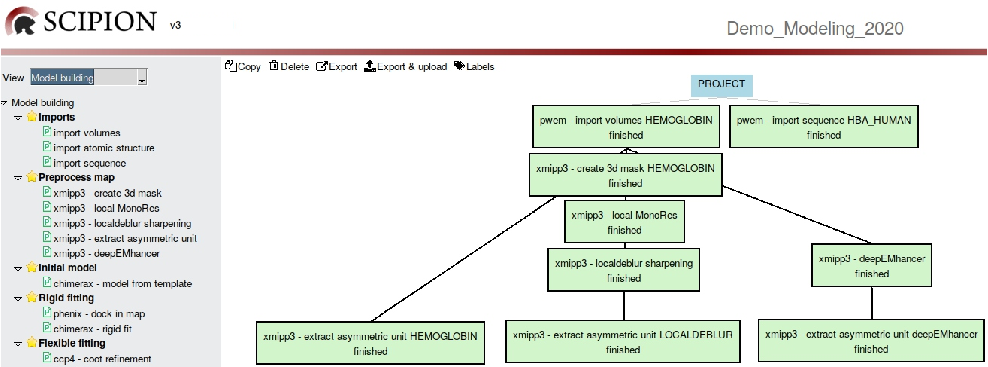
\includegraphics[width=0.95\textwidth]
  {Images/Fig62}
  \caption{\scipion framework detailing the workflow generated after 3D map preprocessing.}
  \label{fig:scipion_workflow_import_2}
  \end{figure}

\subsection*{Map sharpening}
As we have indicated before, since map sharpening contributes to increase  signal at medium/high resolution, we recommend to perform this map preprocessing step before tracing the atomic model of cryo-EM  3D maps \citep{ramirez2018}.  To accomplish this task a couple of automatic alternatives are available in \scipion:  a) local sharpening method independent of initial model, based on local resolution estimation  (\scommand{xmipp3 - localdeblur sharpening} \citep{ramirez2018} (Appendix \ref{app:localDeblurSharpening})), b) deep learning-based sharpening approach (\scommand{xmipp3 - deepEMhancer} \citep{Sanchez-Garcia2020.06.12.148296} (Appendix \ref{app:deepEMhancerSharpening})). 

\subsubsection*{a) Sharpening with $LocalDeblur$}
Since $LocalDeblur$ takes advantage of map local resolution to increase the signal, we have to compute this local resolution as first step to apply the $LocalDeblur$ sharpening method.  Although different algorithms could be used to compute local resolution, we have selected $MonoRes$ \citep{vilas2018}, implemented in \scipion in the protocol \scommand{xmipp3 - local MonoRes}  (Appendix \ref{app:localMonoRes}).\\ 
Since a map binary mask has to be included as a parameter in this protocol, we will build a mask by using the \scipion protocol \scommand{xmipp3 - create 3d mask} (Appendix \ref{app:create3DMask}) as starting step in the local resolution estimation process. Open the protocol form (\ffigure{fig:create3Dmask_1} (1)) and fill in the tap \ttt{Mask generation} (2) with the input volume (3) and the density threshold (4). By default, the level value observed in \chimera main  graphics window (\ffigure{fig:chimera_visualization_volume}) \ttt{Tools -> Volume Data -> Volume Viewer -> Level} can be selected as threshold. In the \ttt{Postprocessing} tap (\ffigure{fig:create3Dmask_1} (5)), select \ttt{Yes} in \ttt{Apply morphological operation} (6) and maintain the rest of options by default. After executing this protocol (\ffigure{fig:create3Dmask_1} (7)), the morphology of the mask generated can be checked in slices by clicking \ttt{Analyze Results} (8).

 
 \begin{figure}[H]
  \centering 
  \captionsetup{width=.9\linewidth} 
  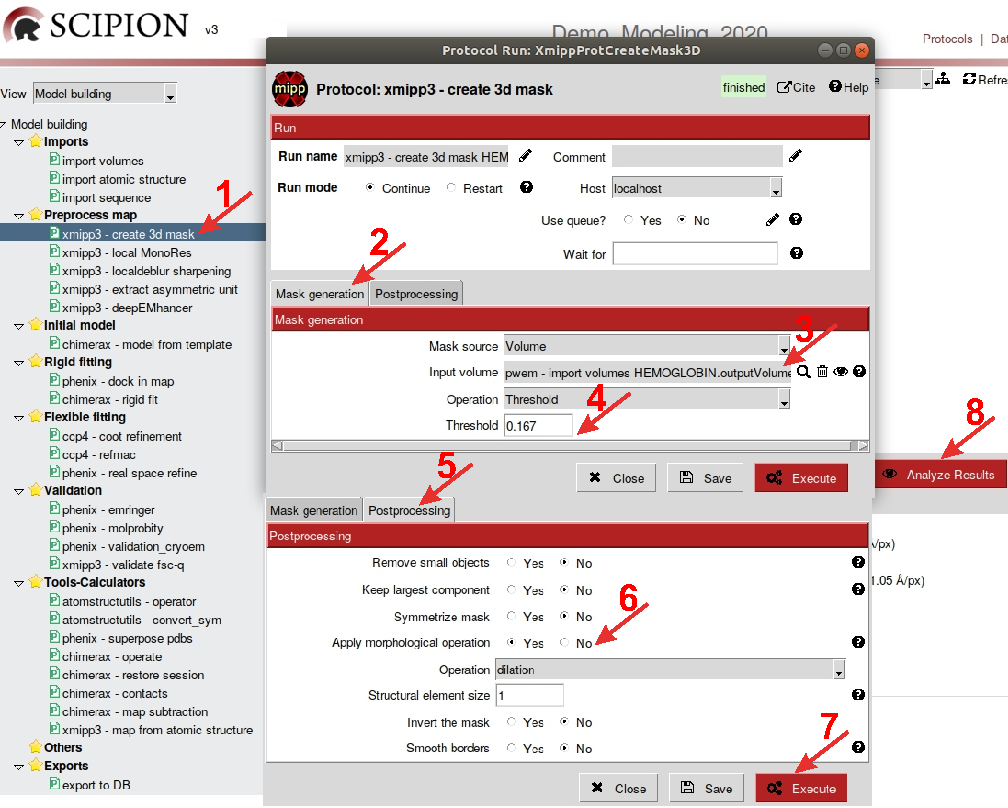
\includegraphics[width=0.95\textwidth]
  {Images/Fig53}
  \caption{Filling in the protocol to create a mask of the initial volume.}
  \label{fig:create3Dmask_1}
  \end{figure}
 
 $ShowJ$, the default \scipion viewer, allows visualize the mask with shape similar to the starting volume (\ffigure{fig:create3Dmask_2}).

 \begin{figure}[H]
  \centering 
  \captionsetup{width=.7\linewidth} 
  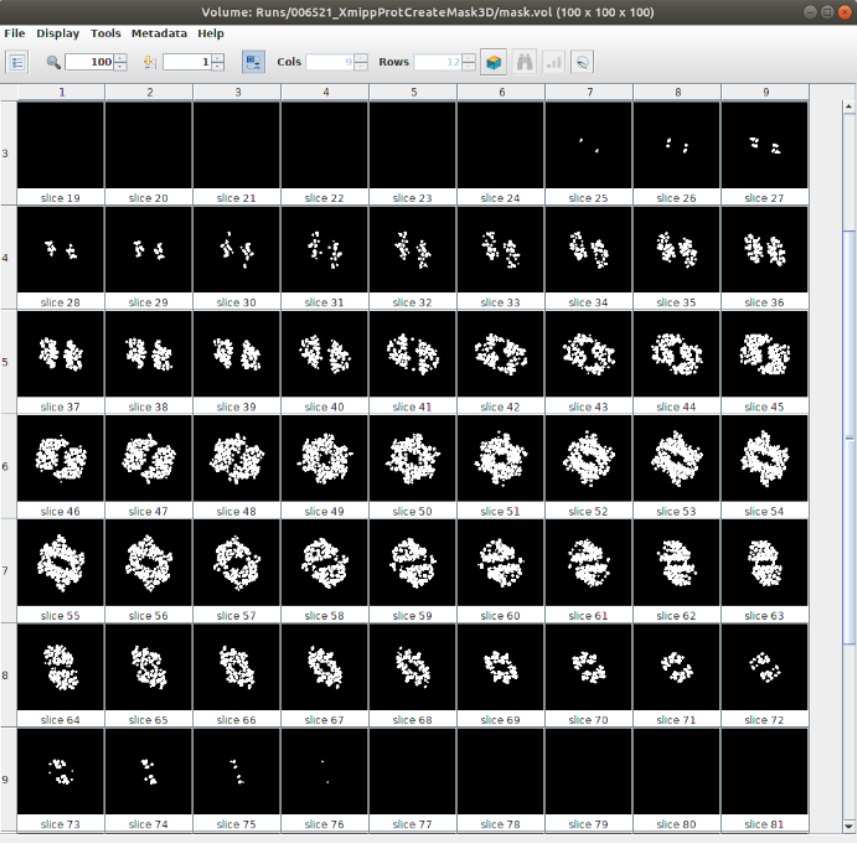
\includegraphics[width=0.60\textwidth]
  {Images/Fig54}
  \caption{Visualizing the mask of the initial volume.}
  \label{fig:create3Dmask_2}
  \end{figure}
  
\ttt{NOTE}: In case you would like to use a previous computed mask, you can do it simply by importing it using the protocol \scommand{import mask} (Appendix \ref{app:importMask}).\\
  
Once the mask of the starting map has been created, the protocol of \scommand{xmipp3 - local MonoRes} can be completed to get the estimation of local resolution. Open the protocol (\ffigure{fig:localMonoRes_1} (1)) and include the starting map (2), as well as the binary mask (3). Finally, based on the map resolution (3.2 \AA), select the default resolution range between \ttt{0.0} and \ttt{6.0} \AA (4). 

\begin{figure}[H]
  \centering 
  \captionsetup{width=.9\linewidth} 
  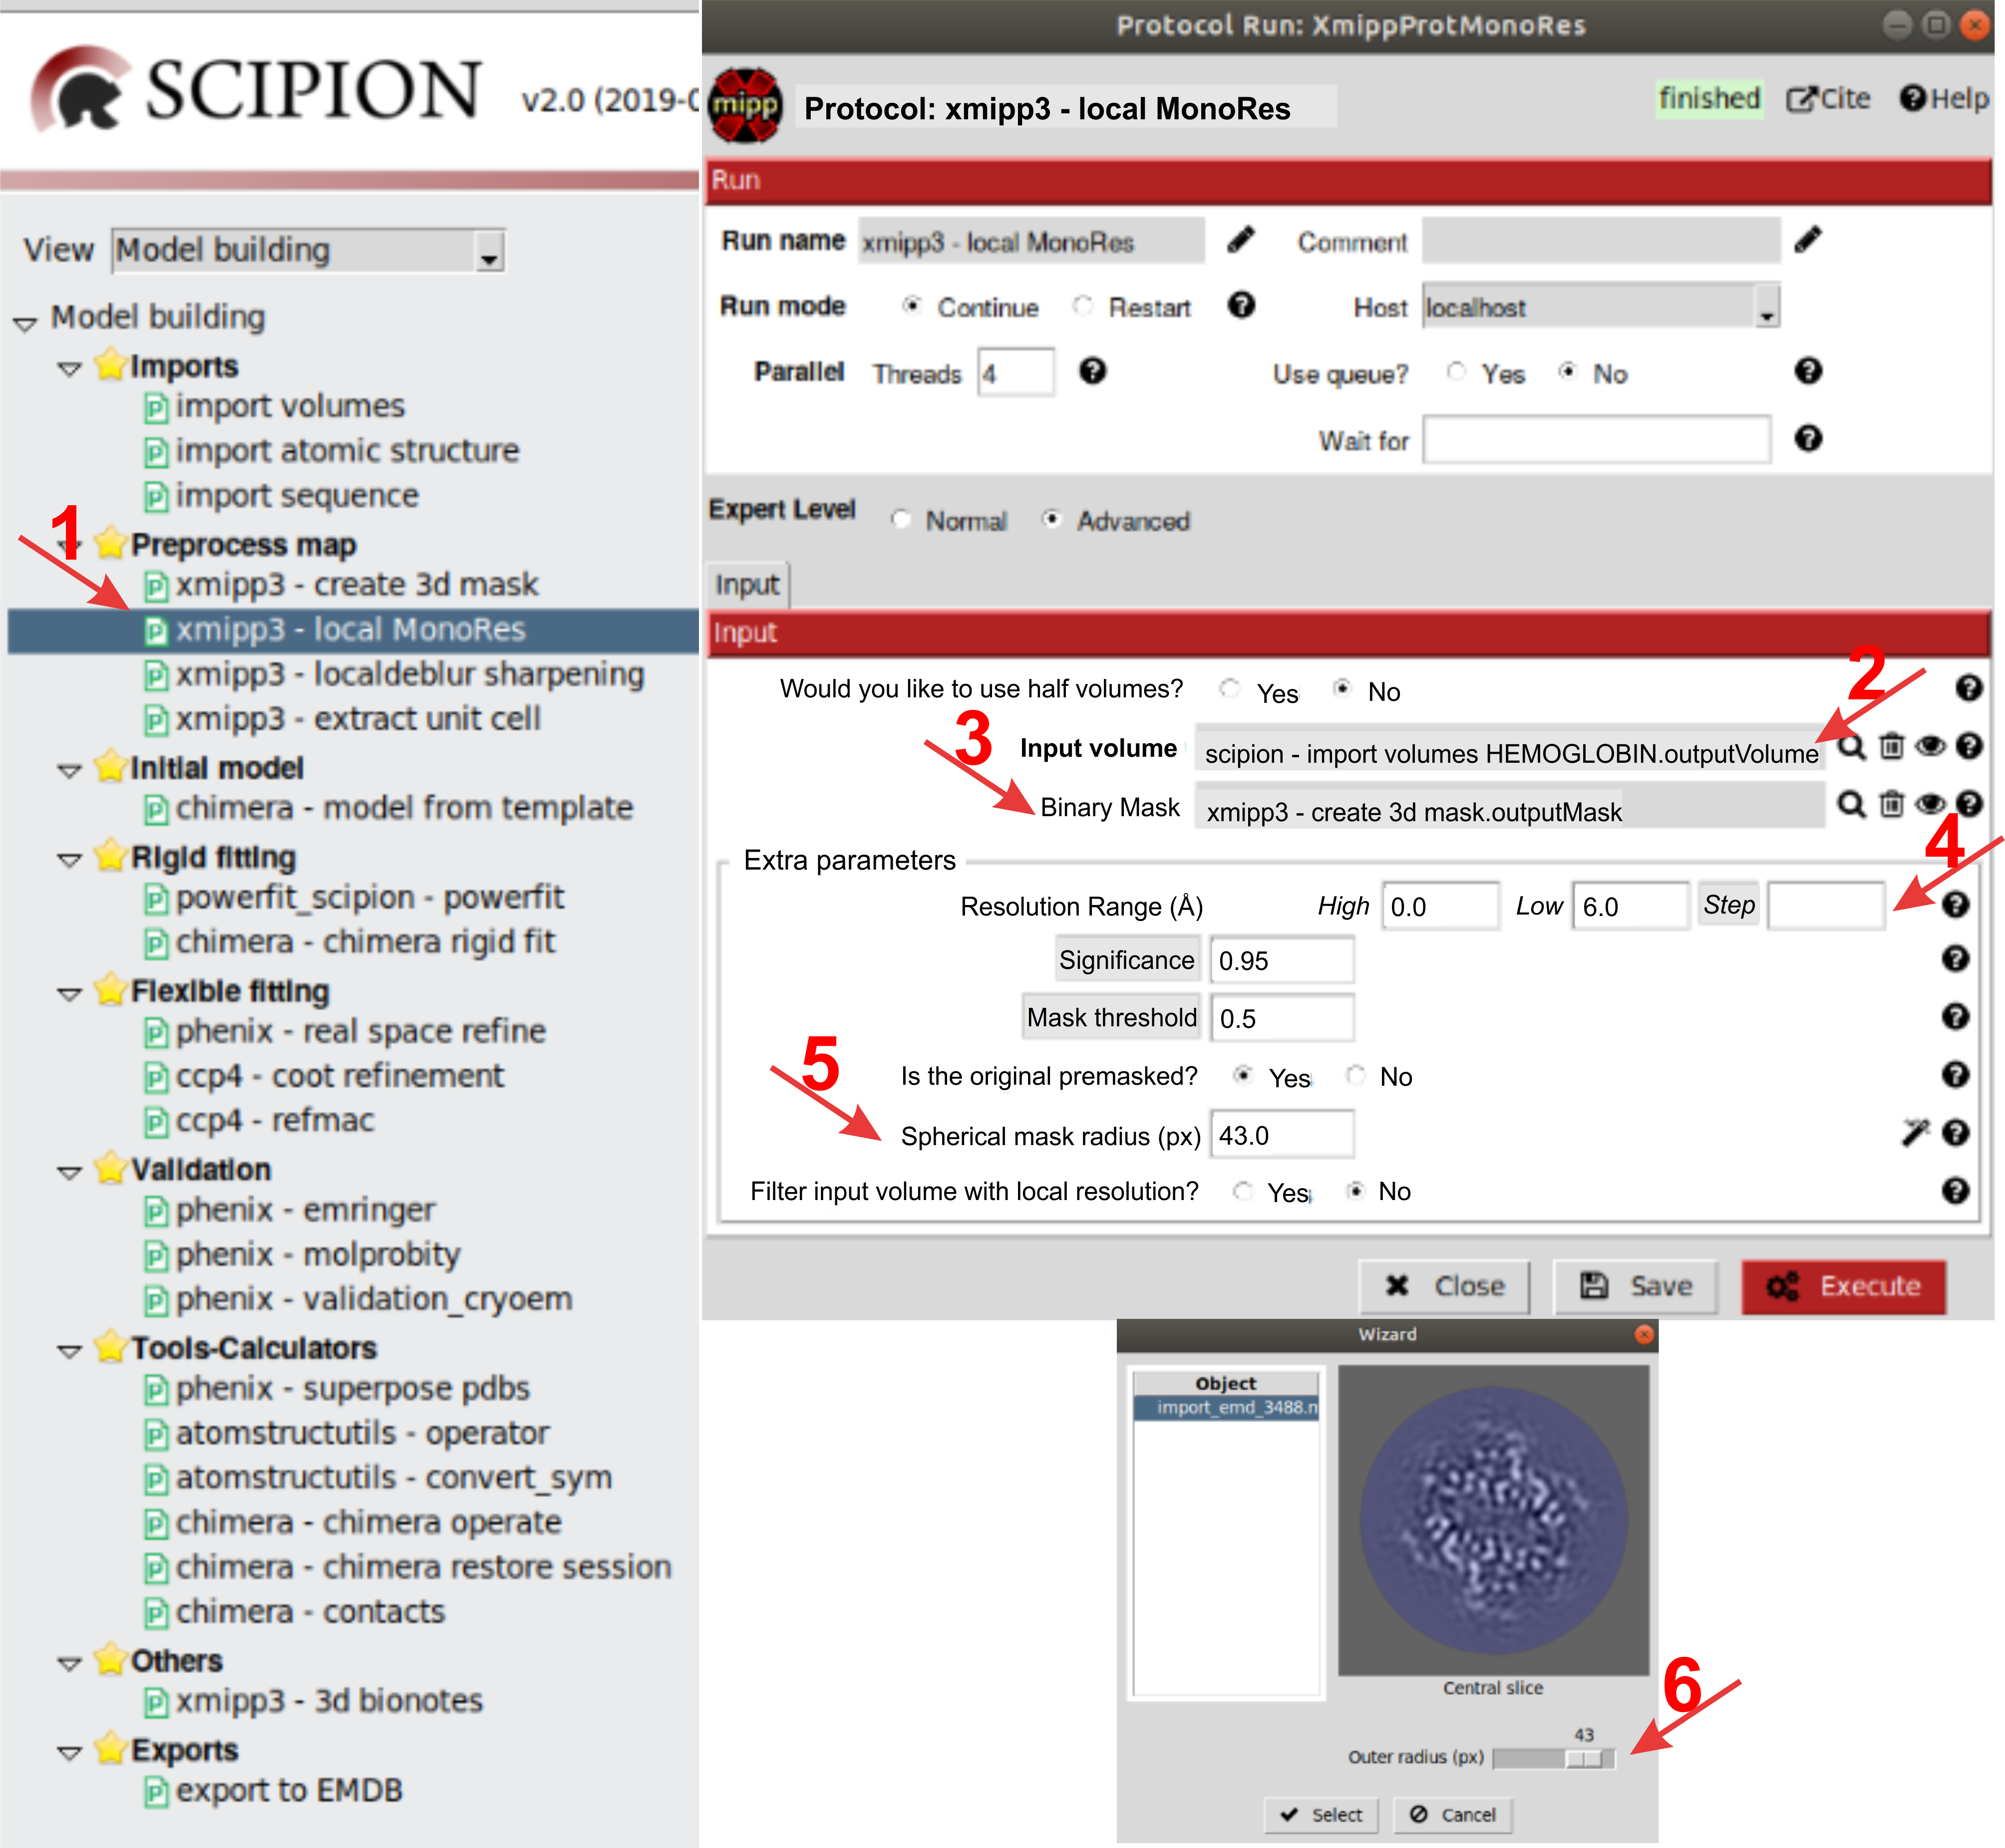
\includegraphics[width=1\textwidth]
  {Images/Fig55}
  \caption{Completing the protocol to estimate the local resolution of the \ttt{metHgb} map.}
  \label{fig:localMonoRes_1}
  \end{figure}
  
Execute this protocol (\ffigure{fig:localMonoRes_1} (5)) and analyze the results (6). The menu of results (\ffigure{fig:localMonoRes_2} (A)), among other views, shows the histogram of local resolutions (1) and the resolution map in \chimera (2). The histogram of resolutions, which displays the number of map voxels showing a certain resolution, allows to conclude that the majority of voxels evidence a resolution between 3.2 and 3.5 \AA, quite close to the published map resolution (3.2 \AA).The resolution map shown by \chimera details the resolution of each voxel (\ffigure{fig:localMonoRes_3}). The bar on the left indicates the color code for resolution values.

\begin{figure}[H]
  \centering 
  \captionsetup{width=.7\linewidth} 
  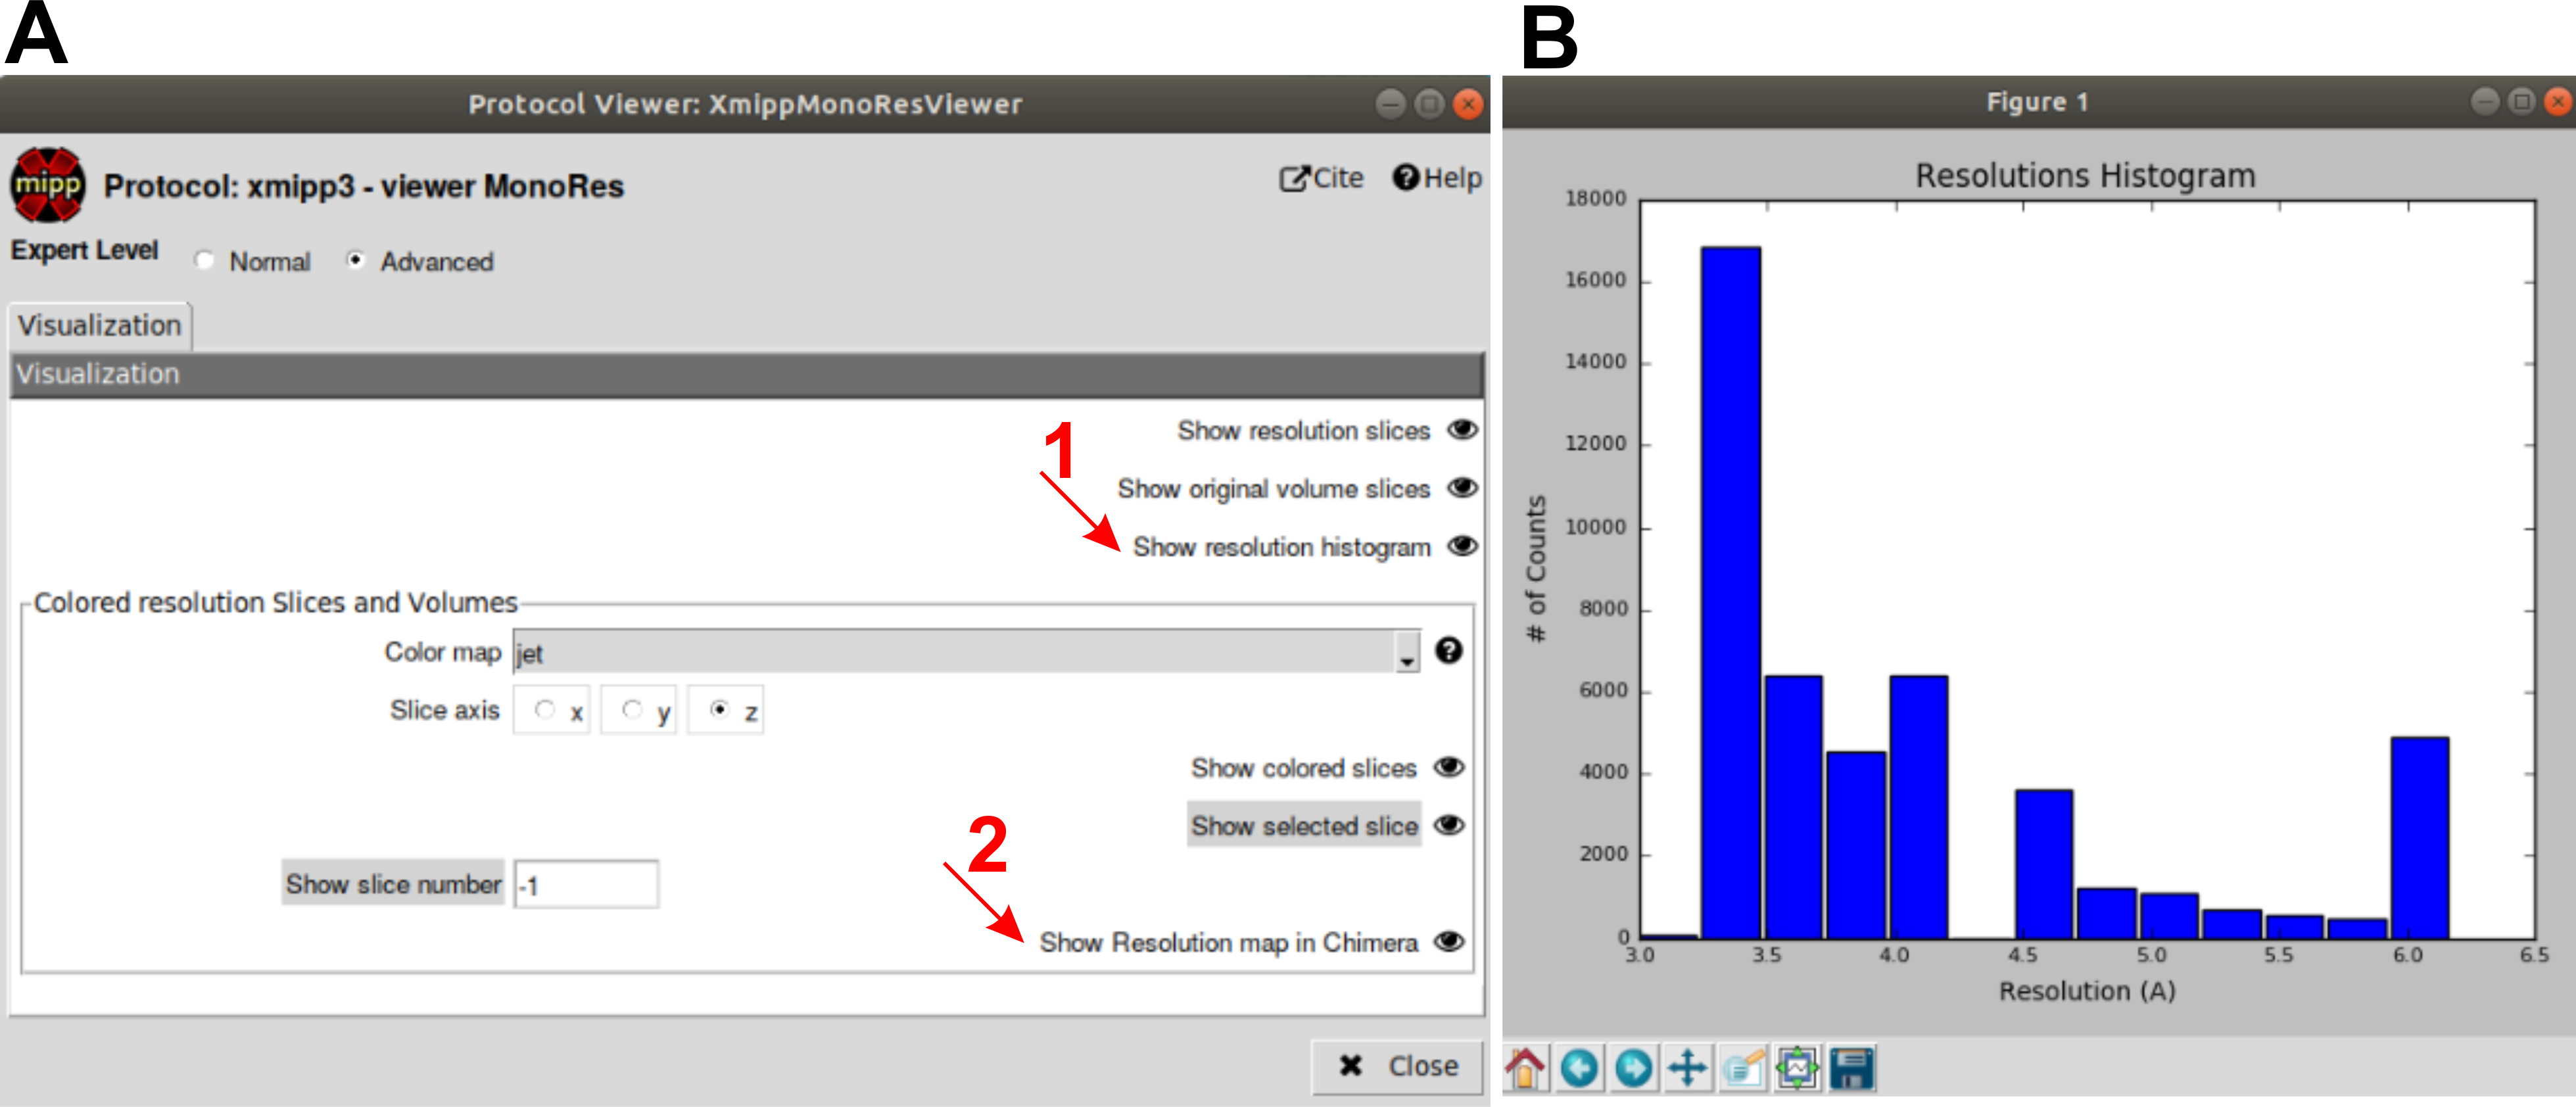
\includegraphics[width=0.80\textwidth]
  {Images/Fig56}
  \caption{\scommand{xmipp3 - local MonoRes} menu of results (A) and histogram of resolutions (B).}
  \label{fig:localMonoRes_2}
  \end{figure}
  
\begin{figure}[H]
  \centering 
  \captionsetup{width=.7\linewidth} 
  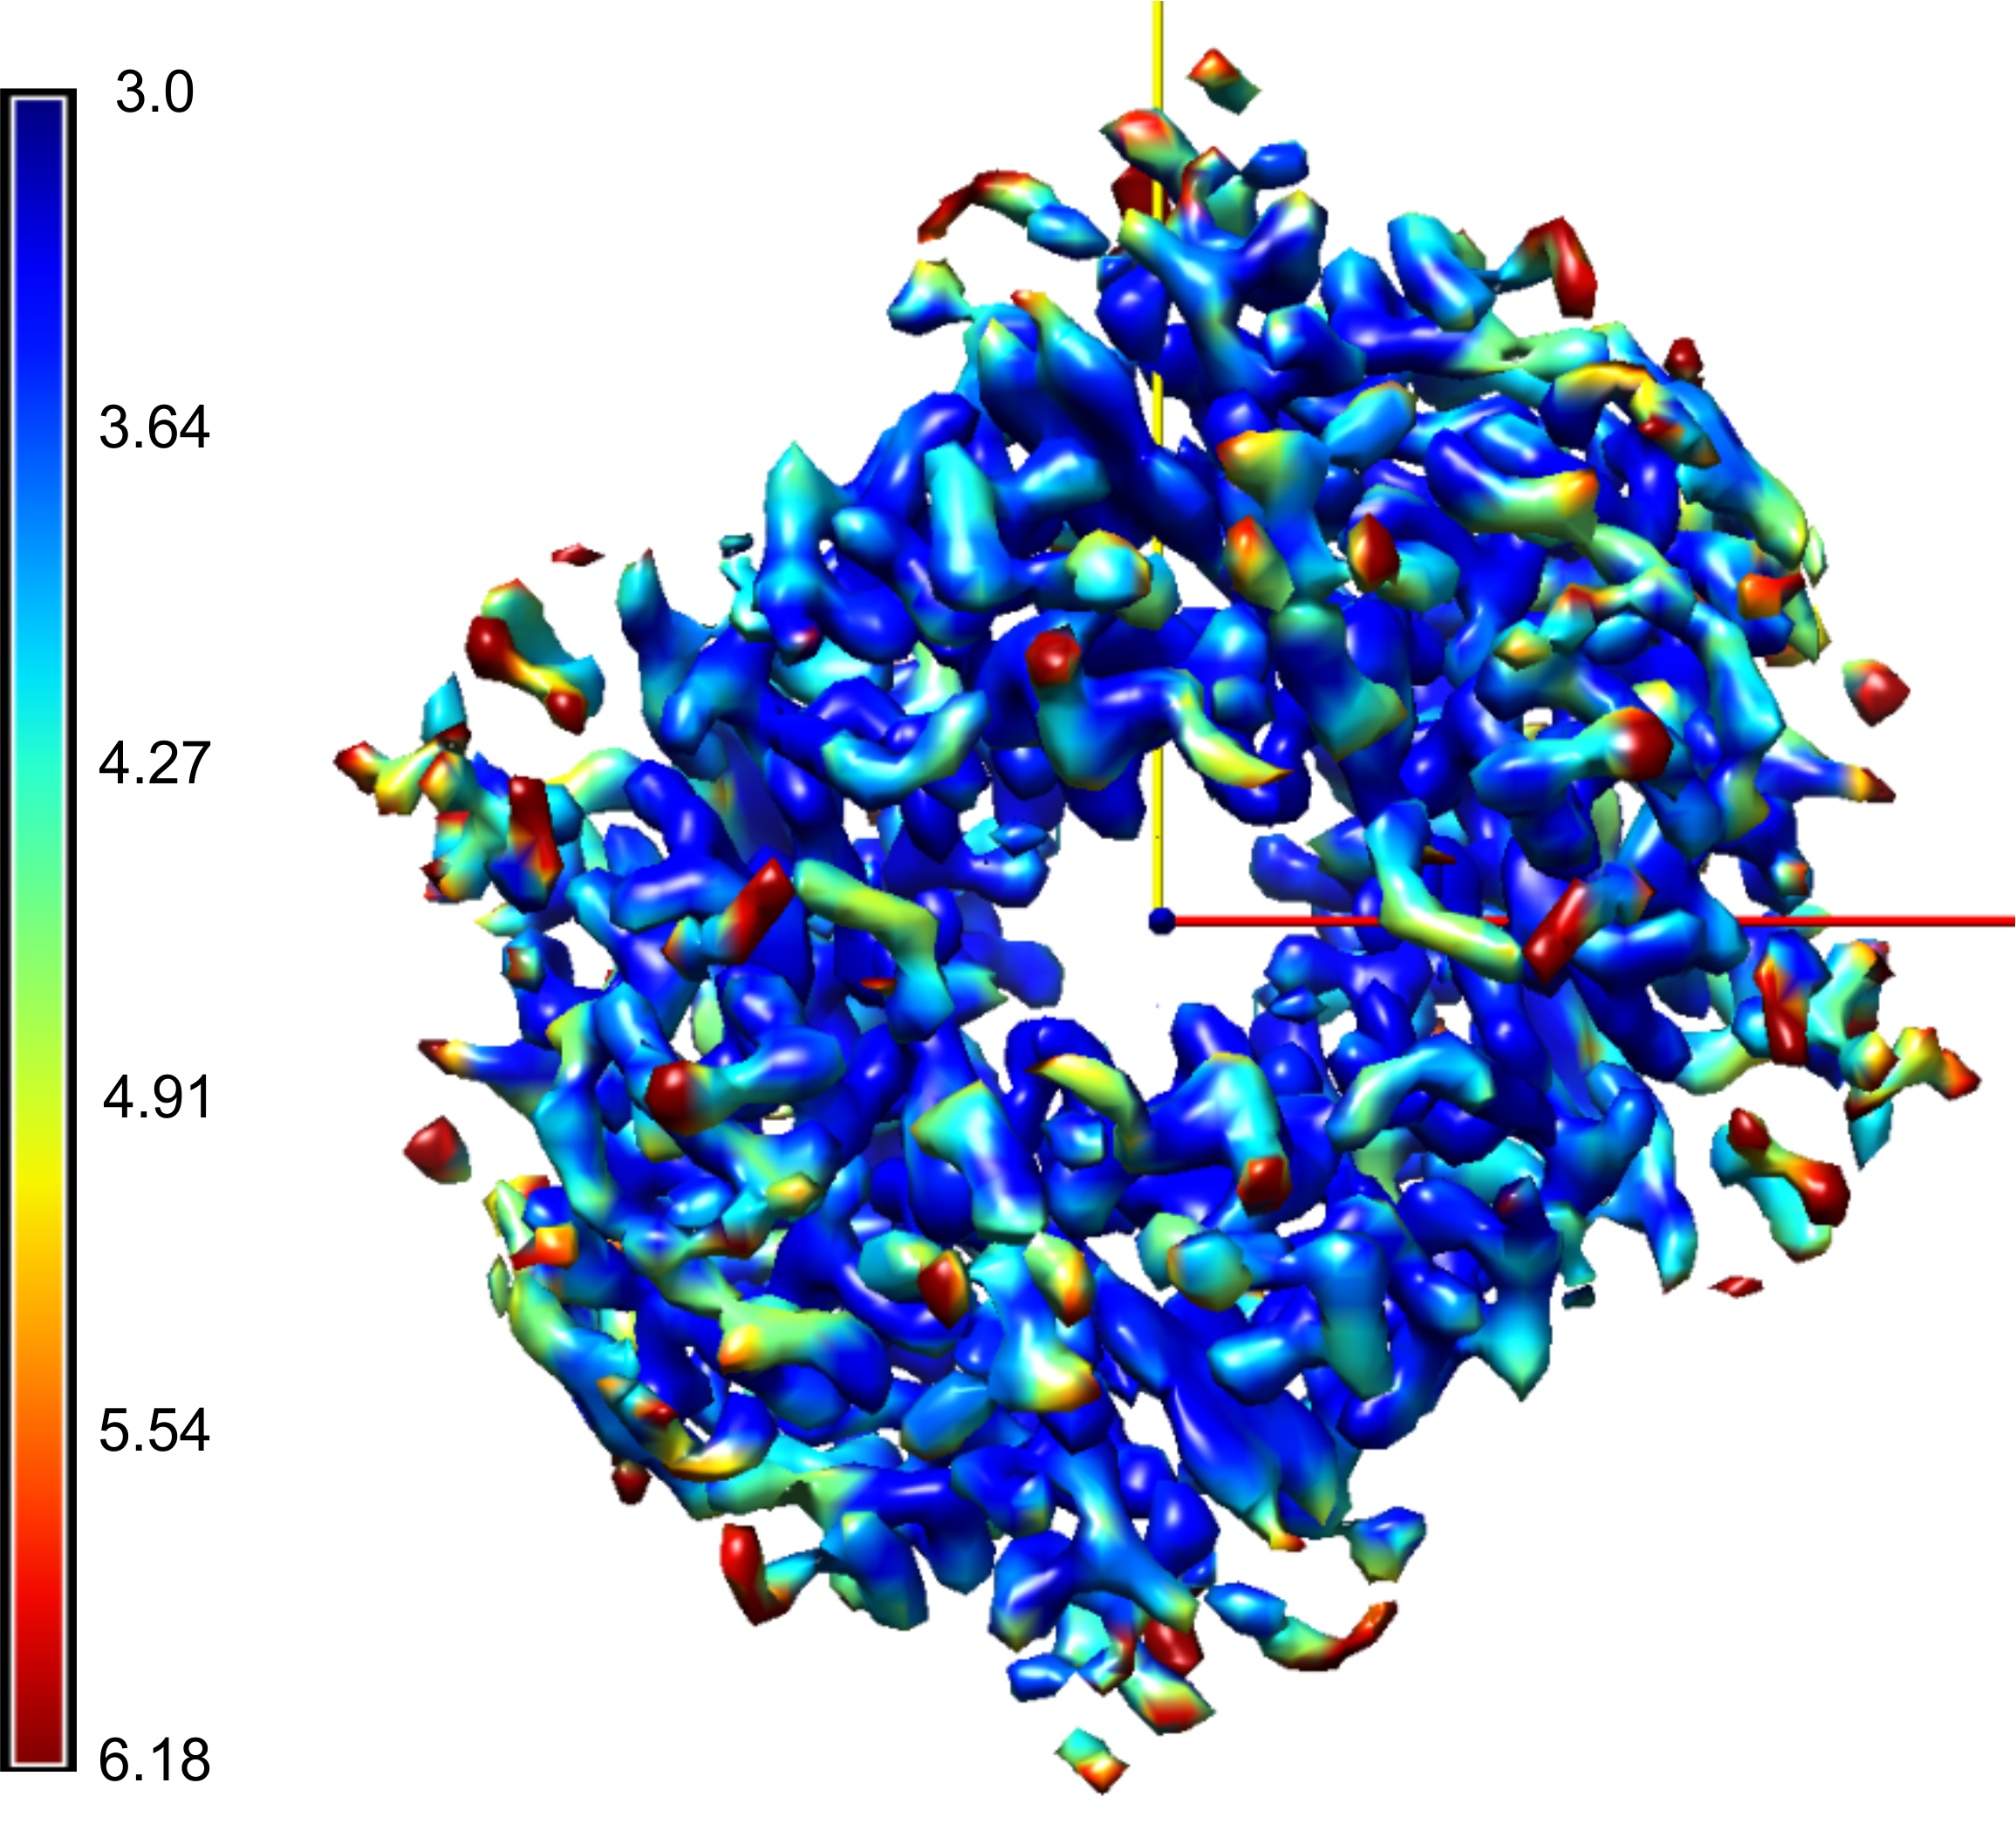
\includegraphics[width=0.70\textwidth]
  {Images/Fig57}
  \caption{Resolution map in \chimera.}
  \label{fig:localMonoRes_3}
  \end{figure}
  
Local resolution values of the input map allow to compute the sharpened map by the \scommand{xmipp3 - localdeblur sharpening} protocol, which implements an iterative steepest descent method that not requires initial model. To accomplish this step, open the protocol (\ffigure{fig:localdeblur_1} (1)) and include the starting map (2) and the map of resolution values (3), maintaining the default values for the rest of parameters (4, 5). 

\begin{figure}[H]
  \centering 
  \captionsetup{width=.9\linewidth} 
  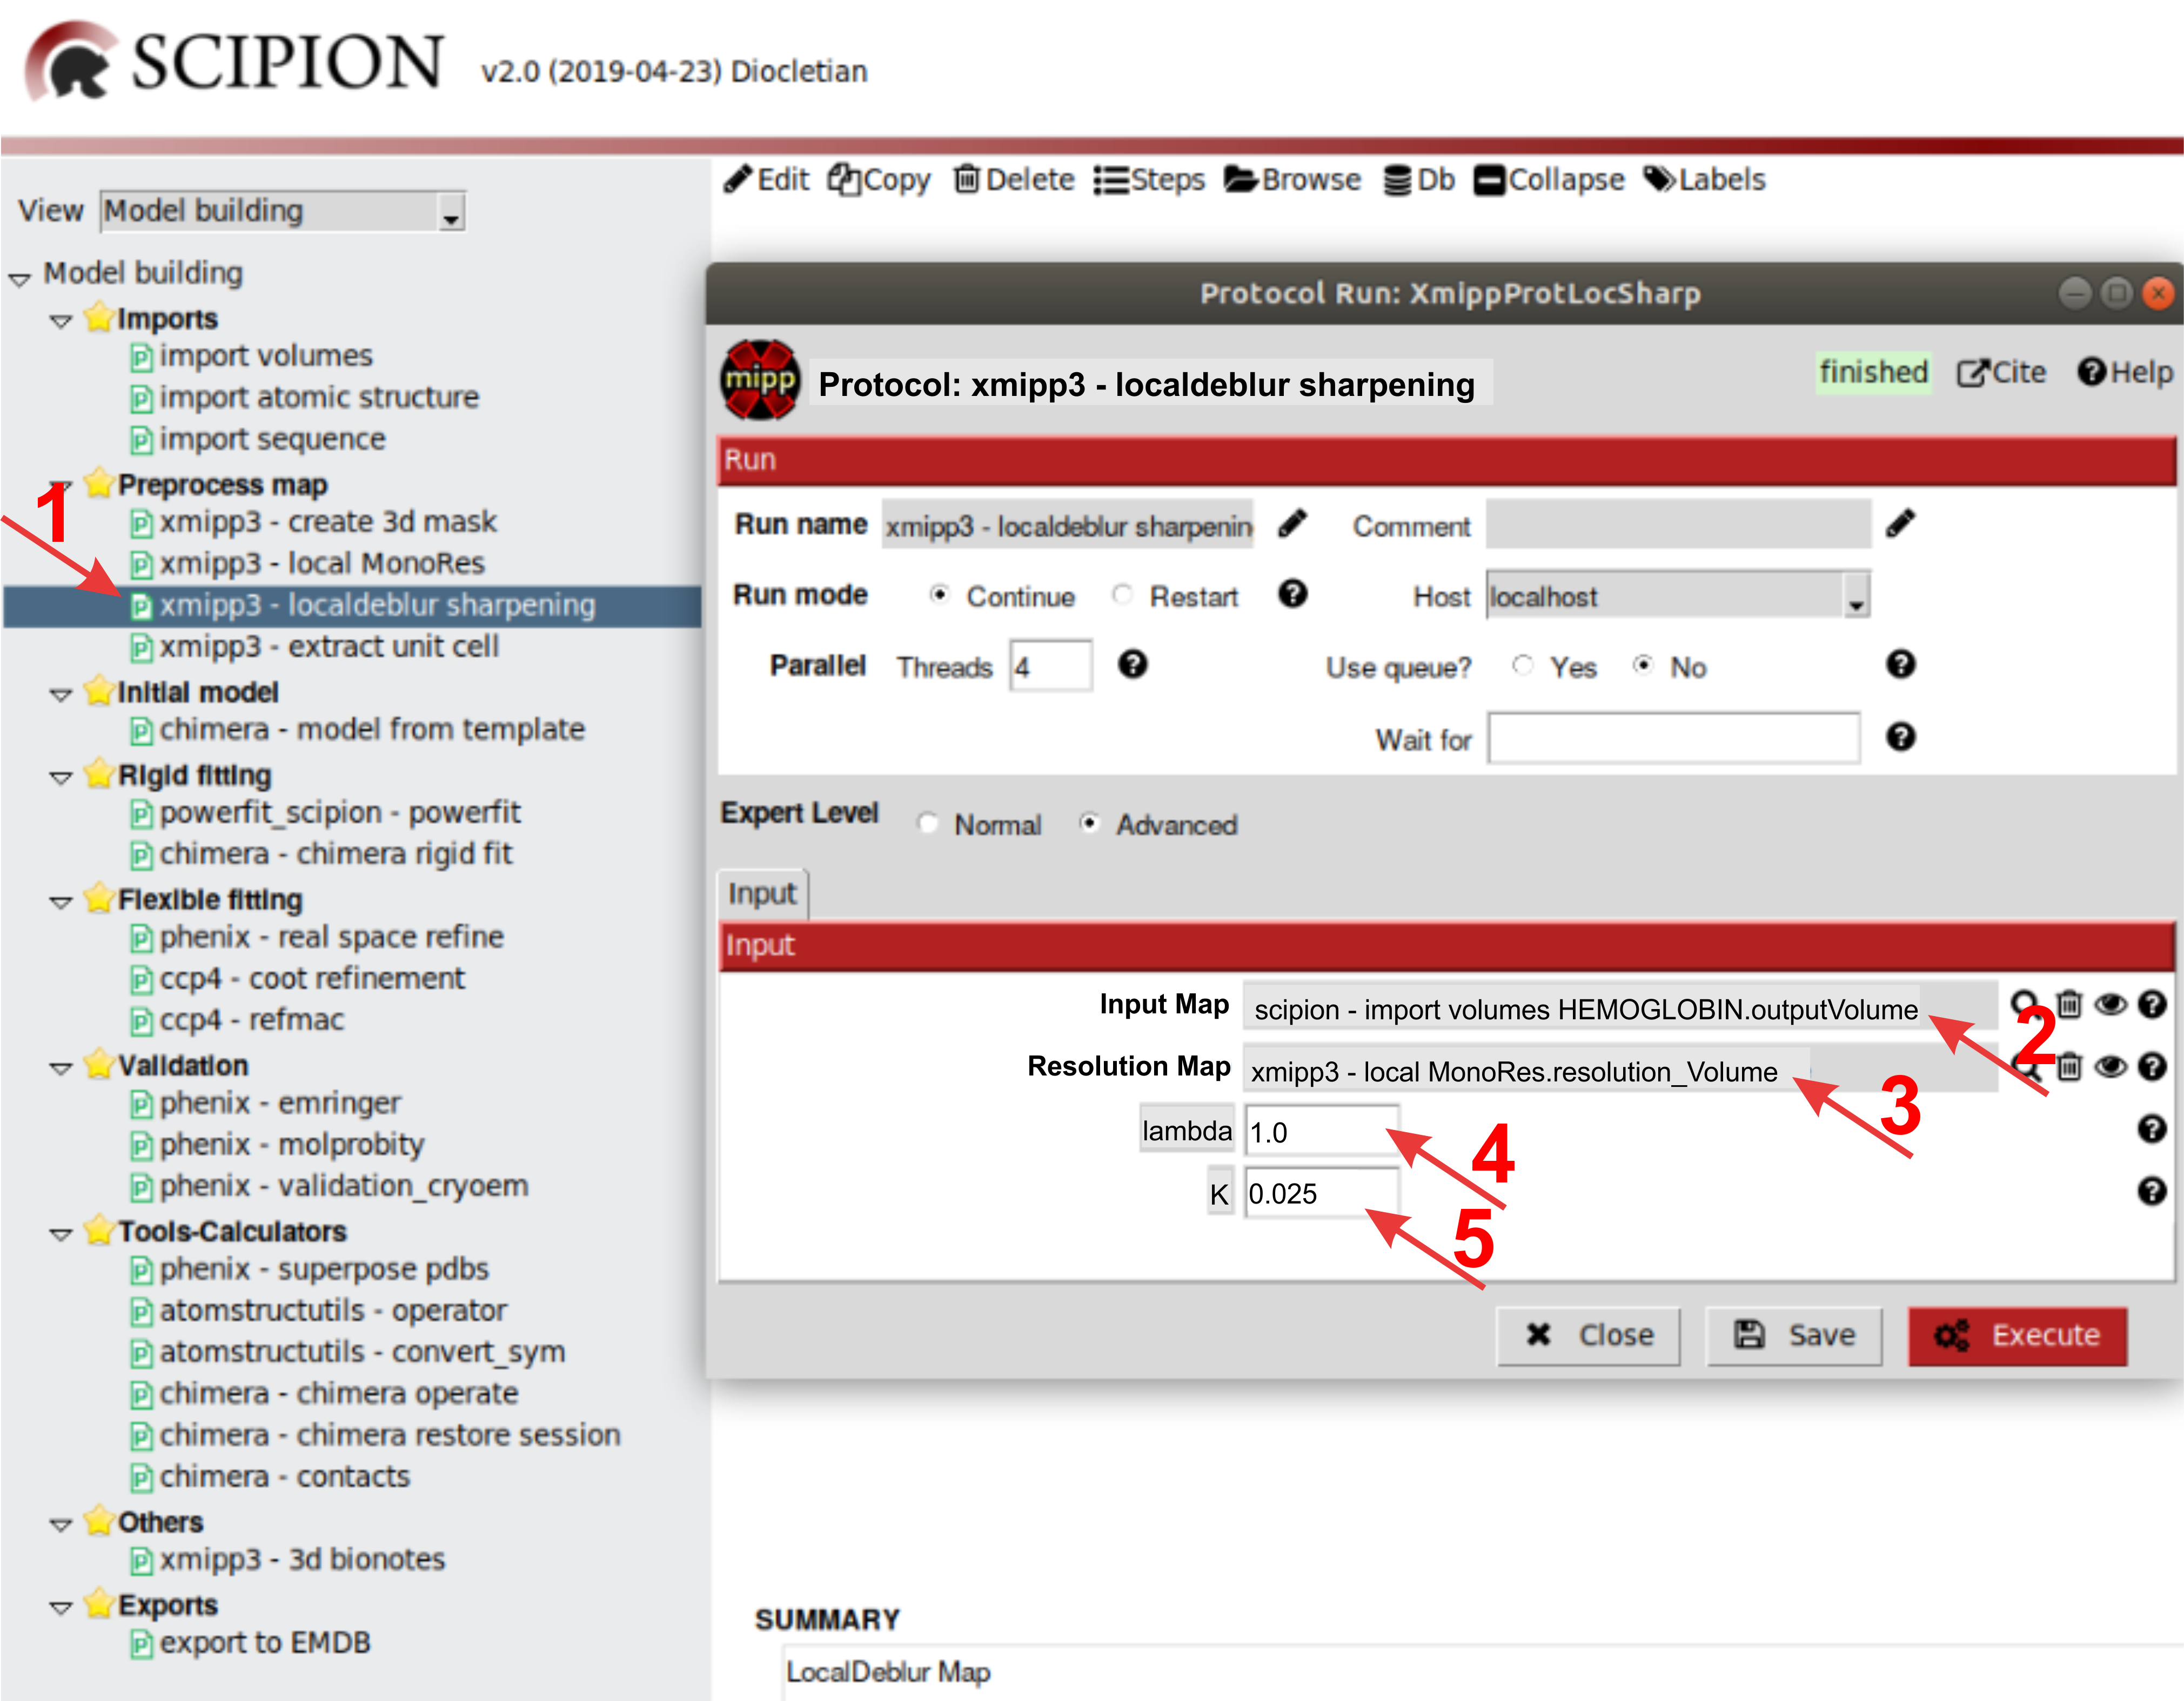
\includegraphics[width=1\textwidth]
  {Images/Fig58}
  \caption{Filling in the protocol to compute the sharpened map.}
  \label{fig:localdeblur_1}
  \end{figure}
  
After two iterations, the sharpening algorithm reached the convergence criterion, $i.e.$ a difference between two successive iterations lower than 1 \%, and stopped. The two maps obtained in the respective iterations can be observed with $ShowJ$ by clicking the black arrow shown in \ffigure{fig:localdeblur_1} (7) with the right mouse botton and selecting \ttt{Open with DataViewer}. Resulting map for each iteration will be shown, as indicated in \ffigure{fig:localdeblur_2}.  Visualization in \chimera is also possible selecting \ttt{Open with ChimeraX} in the menu option \ttt{File} (\ffigure{fig:localdeblur_2} (1)). 

\begin{figure}[H]
  \centering 
  \captionsetup{width=.7\linewidth} 
  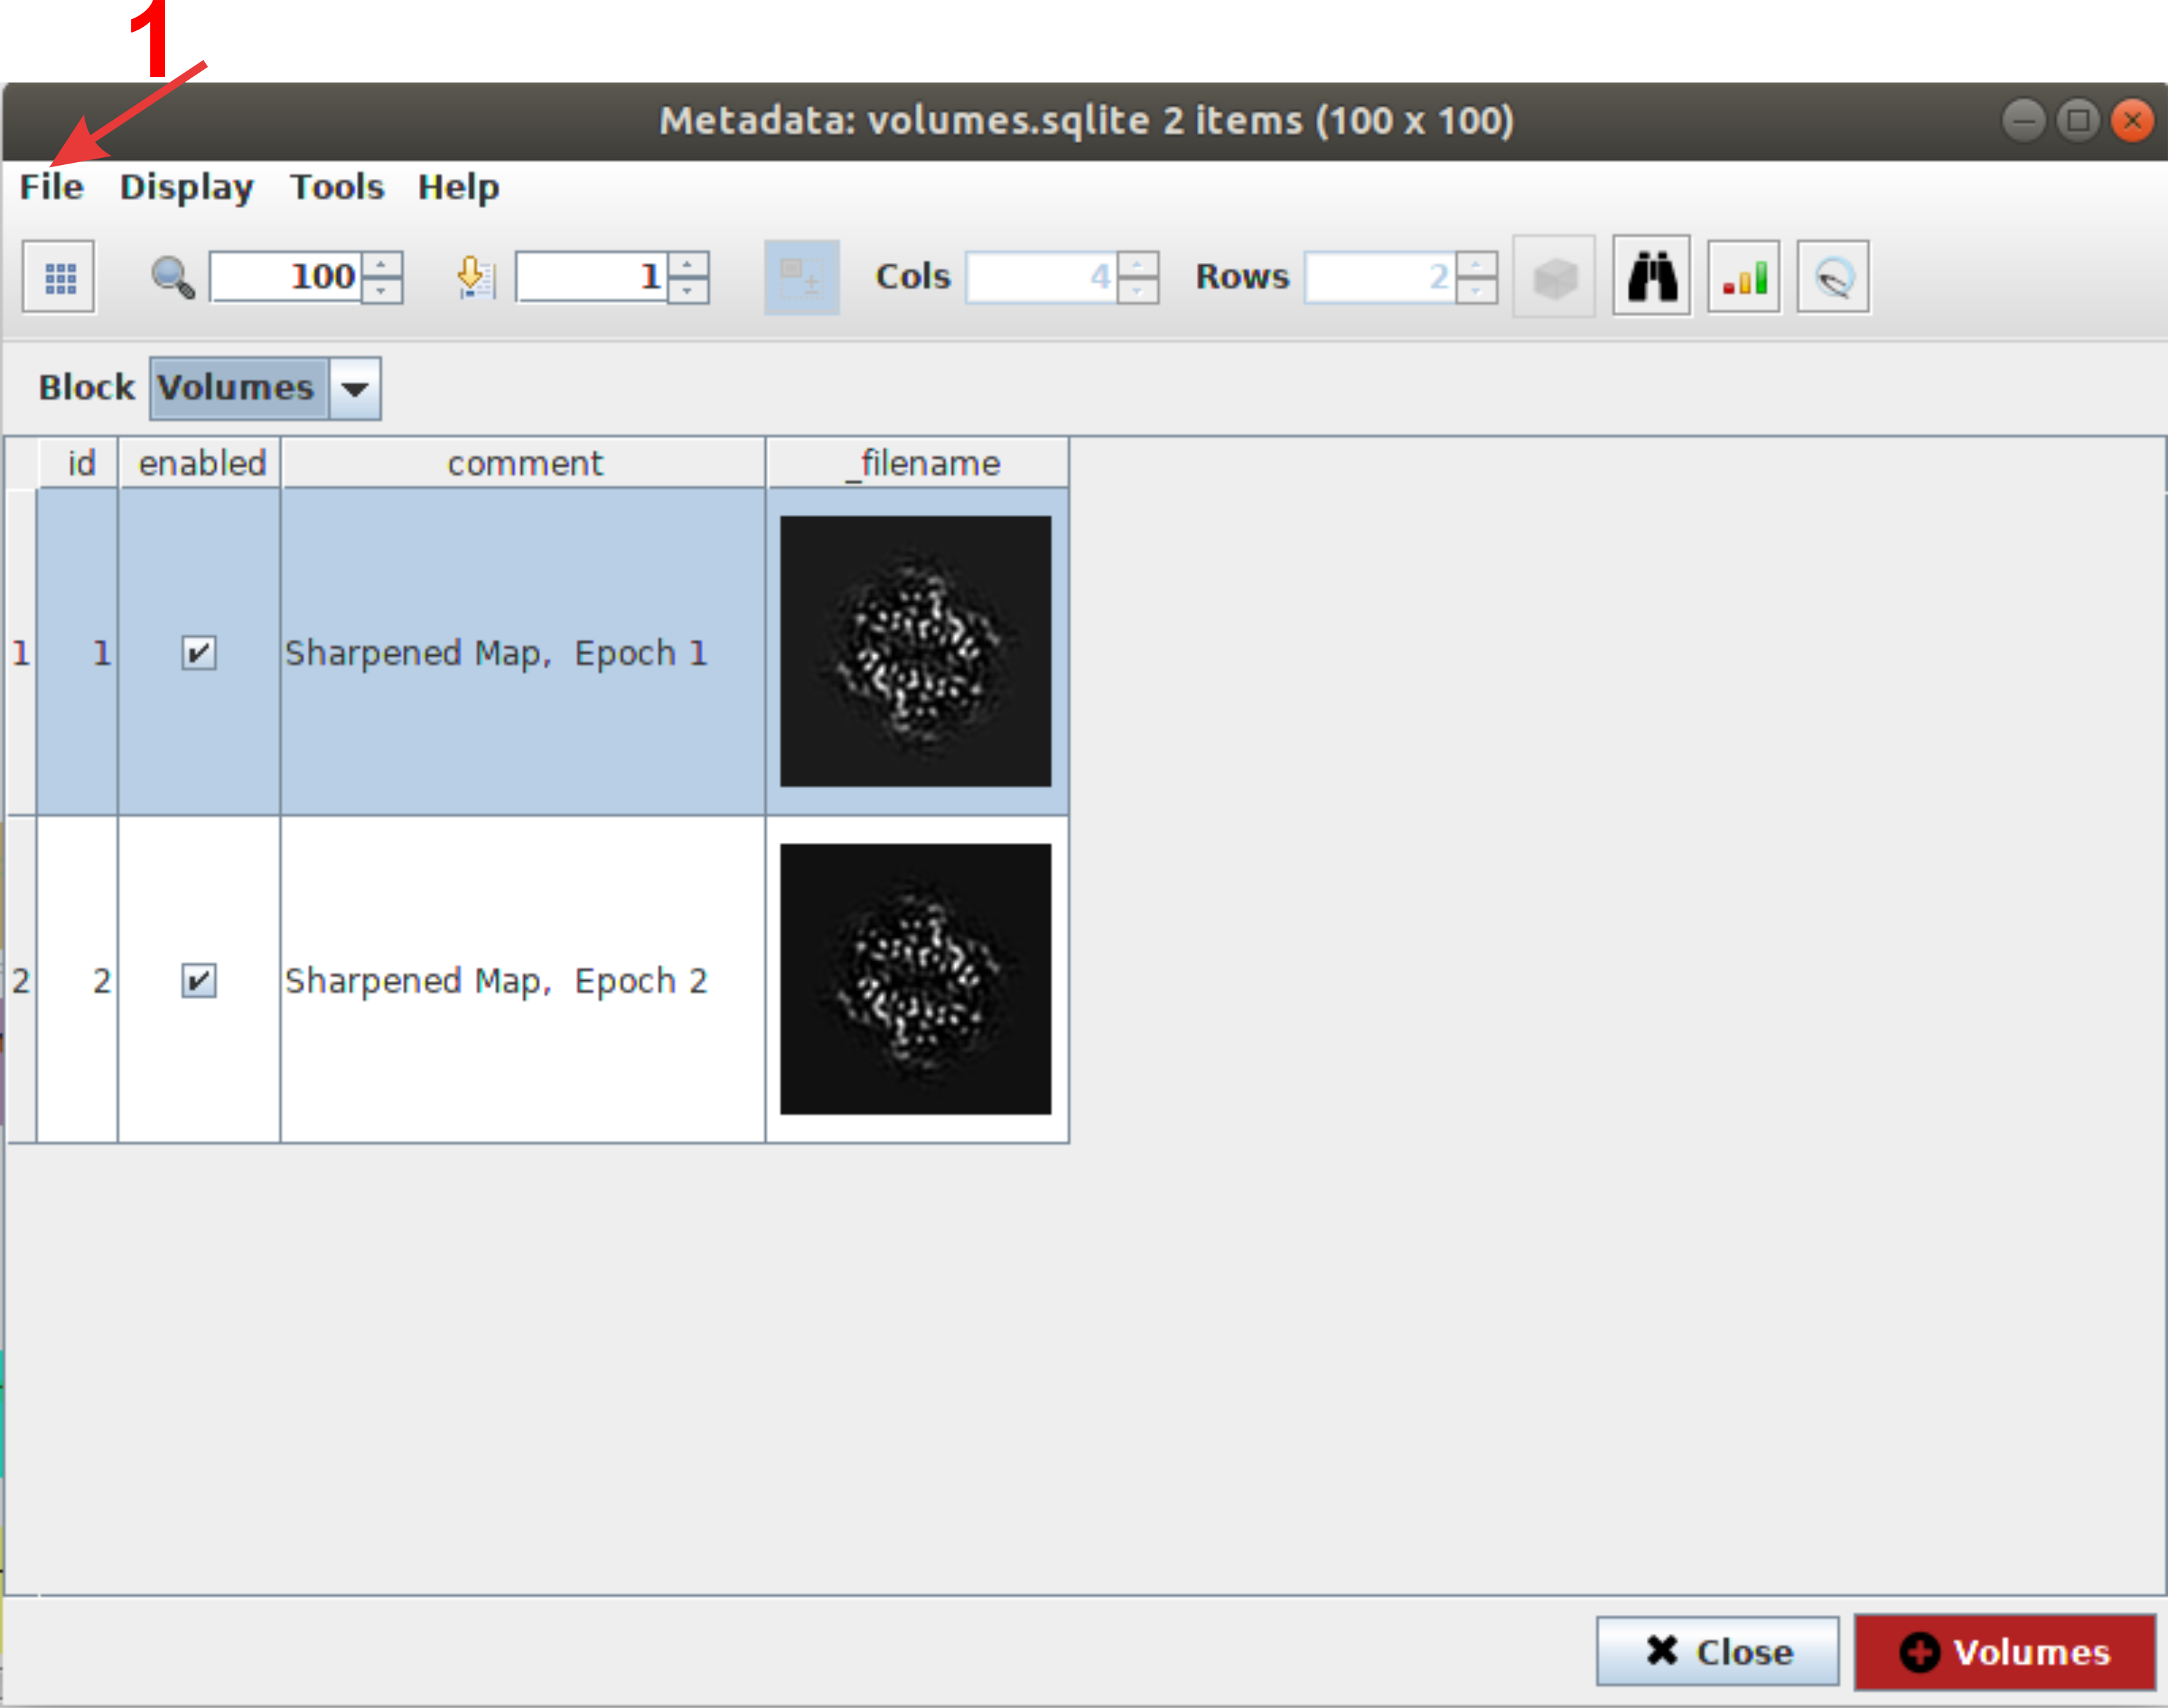
\includegraphics[width=0.65\textwidth]
  {Images/Fig59}
  \caption{Sharpened maps generated after two iterations.}
  \label{fig:localdeblur_2}
  \end{figure}
  
Additionally, by clicking \ttt{Analyze Results} (\ffigure{fig:localdeblur_1} (6)) the sharpened map obtained after the second iteration, $i.e.$ the \ttt{last} map, can be also visualized and compared with the initial one in \chimera (\ffigure{fig:localdeblur_3}).


\begin{figure}[H]
  \centering 
  \captionsetup{width=.7\linewidth} 
  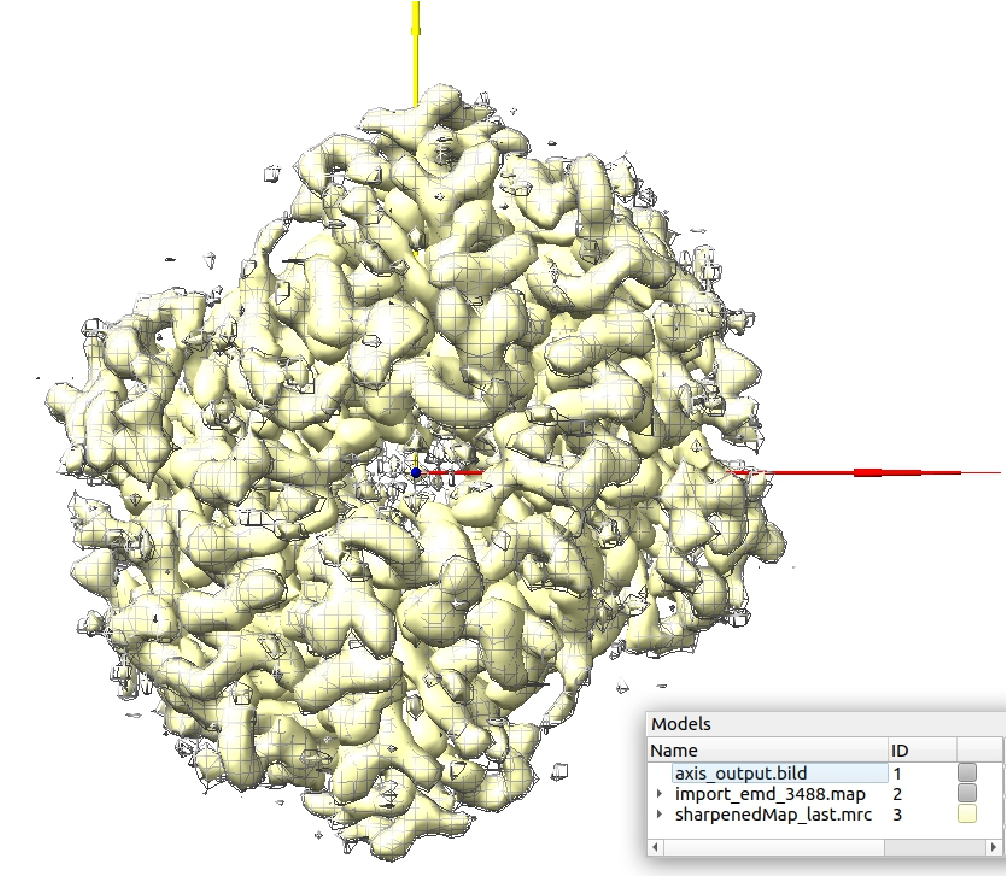
\includegraphics[width=0.65\textwidth]
  {Images/Fig64}
  \caption{$LocalDeblur$ \ttt{last} iteration sharpened map (yellow surface) and input map (grey mesh) in \chimera.}
  \label{fig:localdeblur_3}
  \end{figure}
 
\subsubsection*{b) Sharpening with $DeepEMhancer$}

$DeepEMhancer$ is an alternative automatic sharpening method based on deep learning (\citep{Sanchez-Garcia2020.06.12.148296}), implemented in \scipion in the protocol \scommand{xmipp3 - deepEMhancer} (Appendix \ref{app:deepEMhancerSharpening}). Open this protocol (\ffigure{fig:deepEMHancer_1} (1)) and complete it as indicated. Since only the refined map is available, we are not going to use half maps (2). Include your map (3), the type of normalization desired (4) and the deep learning mode to use (5), in this particular case \ttt{highRes} due to the map high resolution.

 
 \begin{figure}[H]
  \centering 
  \captionsetup{width=.9\linewidth} 
  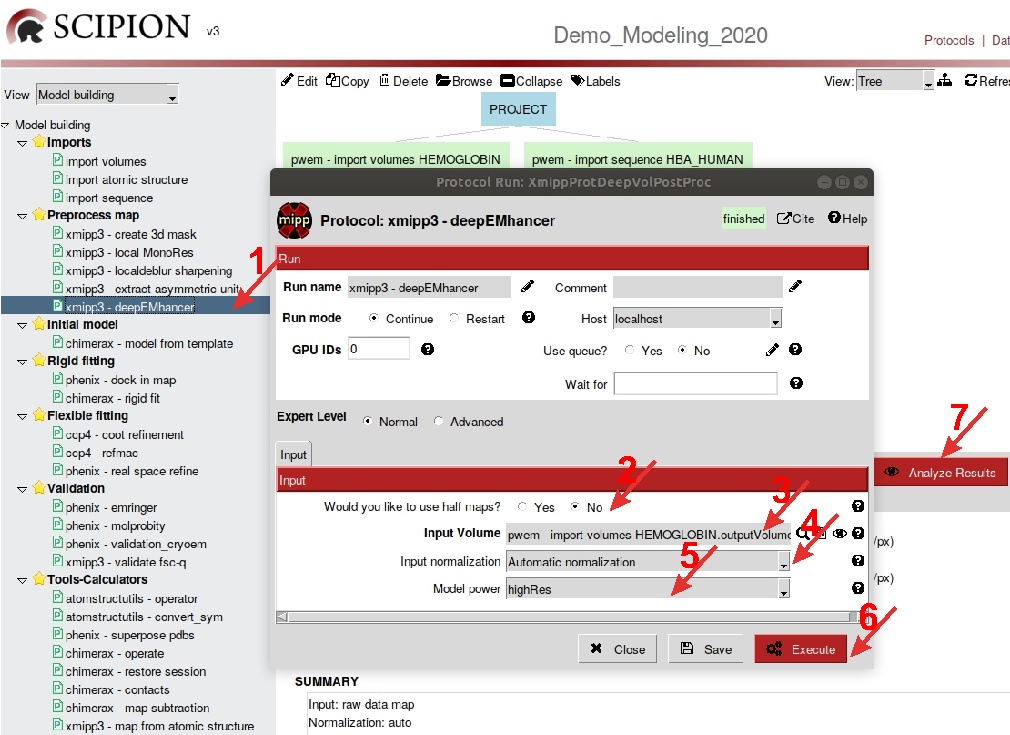
\includegraphics[width=0.95\textwidth]
  {Images/Fig63}
  \caption{Filling in the protocol to generate a sharpened map with $DeepEMhancer$.}
  \label{fig:deepEMHancer_1}
  \end{figure}

After executing the protocol (\ffigure{fig:deepEMHancer_1} (6)), we can check the results (7). \chimera viewer will open and show the sharpened map compared with the initial one (\ffigure{fig:deepEMHancer_2}).

\begin{figure}[H]
  \centering 
  \captionsetup{width=.7\linewidth} 
  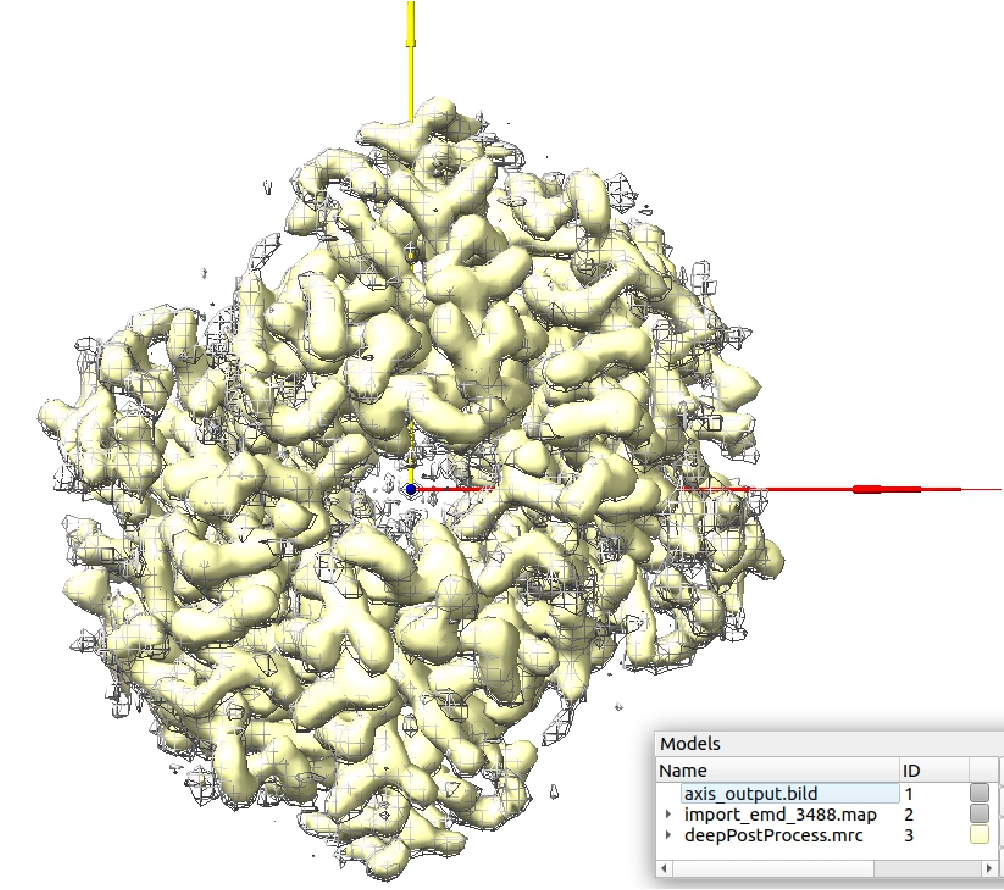
\includegraphics[width=0.65\textwidth]
  {Images/Fig65}
  \caption{$DeepEMhancer$ sharpened map (yellow surface) and input map (grey mesh) in \chimera.}
  \label{fig:deepEMHancer_2}
  \end{figure}
  
\subsection*{Comparison of maps}
Realize that at this point we have generated two optimized maps derived from the initial one. Additionally, some other maps could have been obtained using other map optimization methods. A comparison among them would be interesting to consider which one(s) of them should be used as input in next steps of modeling workflow. The ideal map for tracing the atomic structure should include as many details and connections as possible and, at the same time, preserve the density areas of the initial map. In other words, we can use the best sharpened map (with higher resolution) corroborating that it does not make up new densities, absent in the starting map. Nevertheless, choose ``the best'' sharpened map could be difficult sometimes, especially if the map is very big or there are some regions optimized in one of the sharpened maps and other areas optimized in the other one. In that case, you can use several maps at the same time, having all of them perfectly aligned according to the same origin of coordinates.

In the tiny example shown in this tutorial we are working with a high resolution map and there are almost no differences in resolution between the starting map and the two derived sharpened maps, although this is not usually the case in real life. In this quite uncommon case the initial unsharpened map would be enough to trace the atomic structure. However, in order to detail the method, the starting map and their two sharpened ones will be used simultaneously.




\subsection*{Extraction of the map asymmetric unit}
Since smaller volumes usually include lower number of individual structural elements, making easier fitting models in maps and simplifying modeling process, the part of the map chosen to work with will always be the smaller asymmetrical subunit of the starting loaded map, also known as asymmetric unit (ASU). The size of the ASU thus depends on the symmetry order of the initial volume. The higher the symmetry order, the smaller the ASU. The atomic structure of the whole volume will be obtained straight forward by simply repetition of the ASU structure according to the symmetry order. Then, the first step to simplify the complexity of the initial volume is extracting the ASU. This task can be accomplished by using the \scipion protocol \scommand{xmipp3 - extract unit cell} that extracts the geometrical ASU of the map (Appendix \ref{app:extractUnitCell}).\\

\ffigure{fig:extract_unit_cell} shows how to fill in this protocol form (1). Consider that in this particular case the protocol will be run three times, one with each map (the initial one and the two sharpened derived ones). Include each map in a protocol form parallel to that shown in \ffigure{fig:extract_unit_cell} (2). Since \ttt{metHgb} macromolecule shows symmetry C2, we have selected cyclic symmetry (Cn) as type of symmetry (3), and 2 as symmetry order (4). The angle offset selected (5) turns -45º around the Z axis the mask used to create the ASU. 
%Remark the relevance of including the offset in order to extract a unit cell able to reconstruct by symmetry the whole volume regarding the symmetry axes. 
The two wizards on the right (6, 7) help you to select the radii to delimit a fraction of the map comprised between the coordinate origin (inner radius 0.0) and the maximum radius (outer radius 50.0). The final extracted volume will be slightly higher than the ASU due to the expand factor 0.2 (8). % We use an expanded unit cell  to favor the modeling of each individual structure edges. 
The respective tutorial appendix \ref{app:extractUnitCell} includes a comprehensive explanation of the meaning of parameters. 

 \begin{figure}[H]
  \centering 
  \captionsetup{width=.9\linewidth} 
  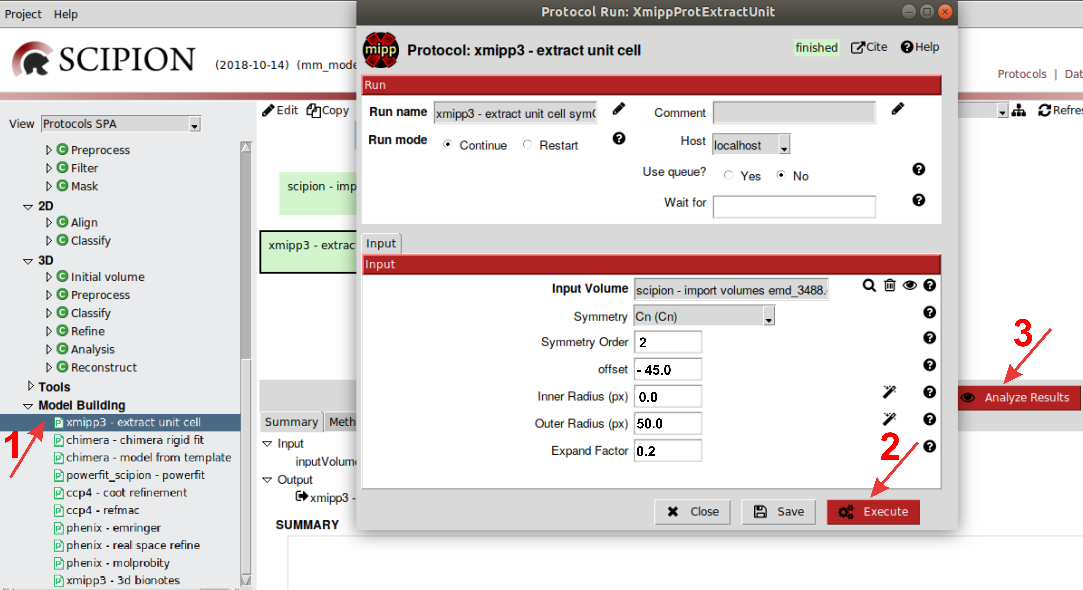
\includegraphics[width=1\textwidth]
  {Images/Fig7}
  \caption{Extracting the map asymmetric unit (ASU).}
  \label{fig:extract_unit_cell}
  \end{figure}
  
After executing the protocol (\ffigure{fig:extract_unit_cell}(9)), the resulting expanded ASU can be observed (10) with \chimera (\ffigure{fig:chimera_visualization_unit_cell}). Note the additional expanded volume of the  ASU on the left side of the figure. The ASU itself, on the right side, constitutes the half volume. Since the total volume contains the structure of four proteins, we can anticipate that this smaller asymmetrical subunit of the initial volume contains two proteins, one $\alpha$ and one $\beta$ \ttt{metHbg} subunits. Then, the respective structures of these two proteins could be fitted in the map ASU simultaneously or in successive modeling workflow steps. 
  
 \begin{figure}[H]
  \centering 
  \captionsetup{width=.7\linewidth} 
  \includegraphics[width=0.80\textwidth]
  {Images/Fig8}
  \caption{Expanded ASU (yellow-green-blue) and initial volume (gray) visualized with $ChimeraX$. The purple broken line on the right delimits the ASU (right) and its expanded volume (left).}
  \label{fig:chimera_visualization_unit_cell}
  \end{figure}
